
%---------------------------------------%
% Packages arranged by : Tsz Timmy Chan %
%                 Date : May 26th, 2019 % 
%---------------------------------------%

\documentclass{TC}
\usepackage{TCcommon}

\title{TITLE HERE}	% Work Title Here.
\author{Tsz Timmy Chan}	% YOUR NAME HERE 

\usepackage[notes]{TCheader}
\usepackage{TCexamtitle}

\usepackage{setspace}
\linespread{1.5}

%\renewcommand{\benediction}{" " - }
%\renewcommand{\quoteoftheday}{" " \\ - }

\begin{document}
Student Led Discussions: 
Notes by Timmy Chan, Mee Na Feng, Sidney Spurgeon:

\begin{itemize}
\item Overview: Discourse can be considered in multiple formats and mediums. Discourse can be embodied in "spoken/signed" form and received in the action of  "listening/seeing/feeling", or encapsulated in "written" form either visually or in braille, and received in the action of "reading".
\item Key Takeaways: Discourse through text and discourse through dialogue are inherently different. 
\begin{figure}[H]
\centering
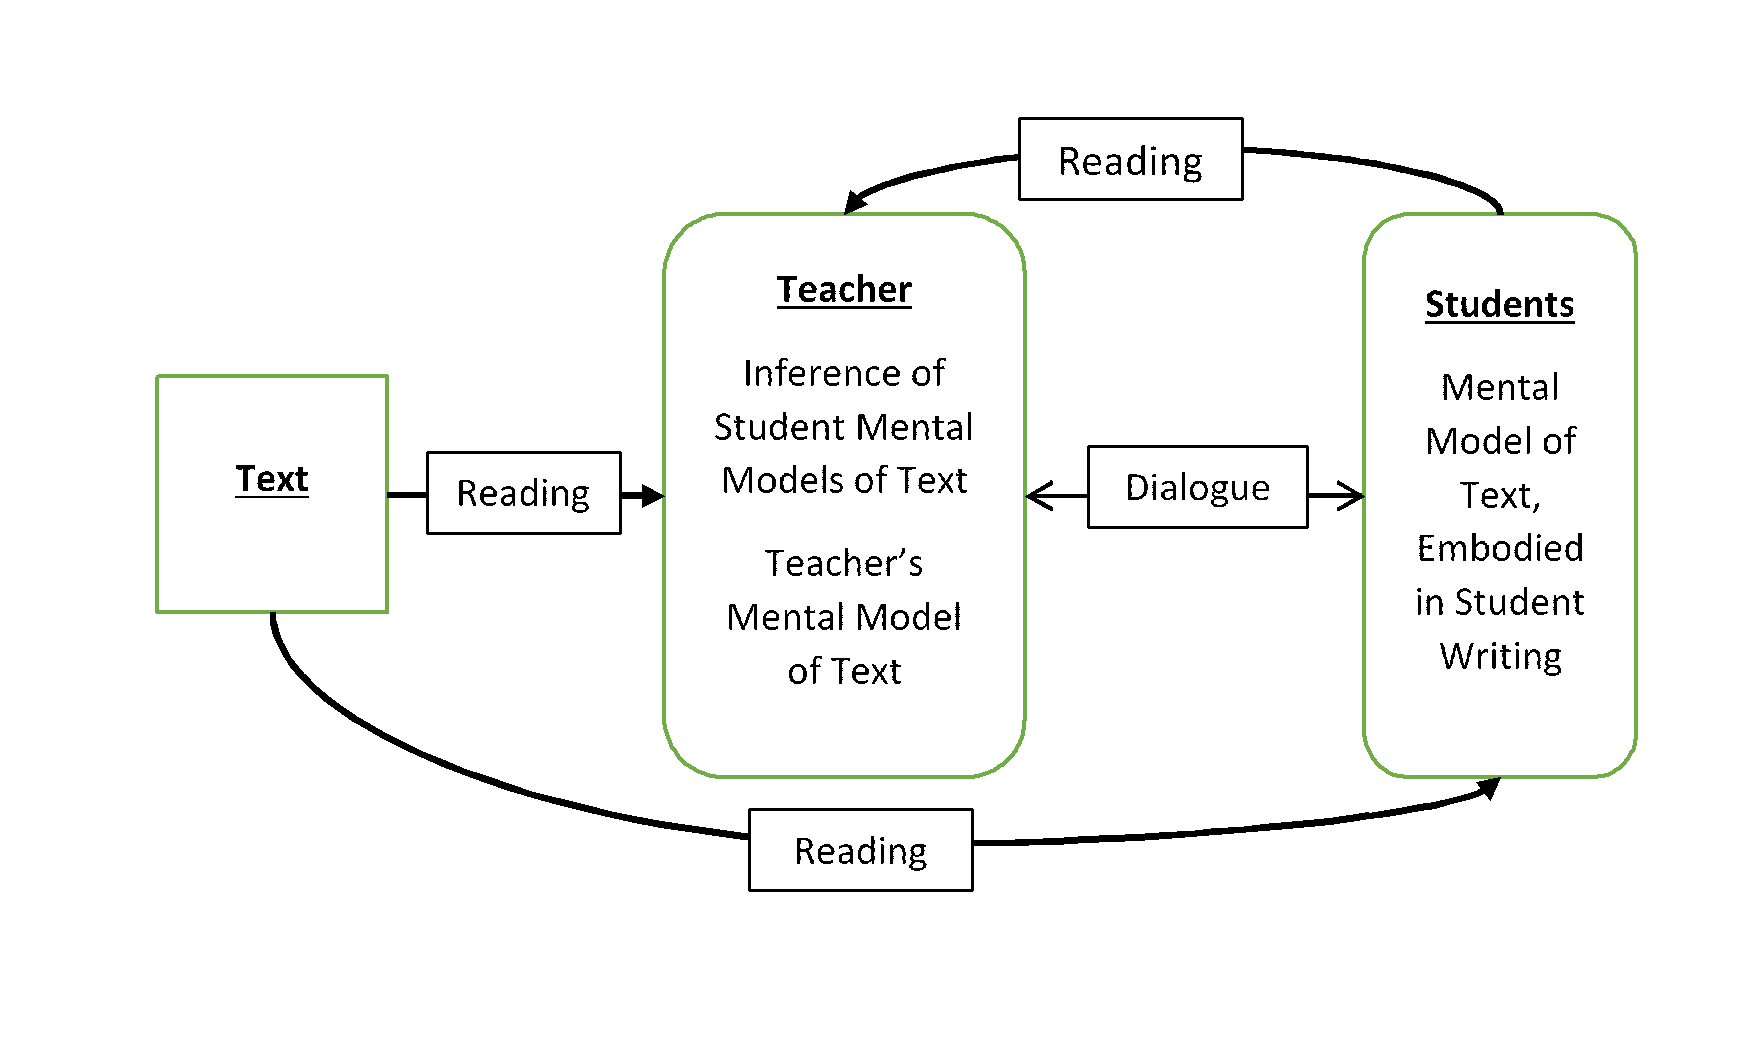
\includegraphics[width=.75\textwidth]{Discourse_I_diagram}
\caption{diagram, susan noted the top arrow should be "writing"}
\end{figure}

\item Relationships to Topic Area and/or Research Methods: Just as with other methodologies, discourse analysis can be tailored to fit the needs of the researcher in answering their research question(s). Some forms of discourse analysis may not fit the particular setting or materials being researched. The type of analysis may also be too narrow, or inversely too broad, to effectively and reliably answer the research question. 

\end{itemize}
Discourse Analysis: Written text. \parencite{goldman_discourse_2011}
\begin{itemize}
\item Summary: Abstract:
Established that there exists a need for a better metric for analyzing the complexity of text than the formulas that exist, and leads to the concept of cohesion.

This chapter seems to serve as a gateway to written text discourse analysis. The article demonstrates how discourse analysis can be used to analyze many different types of text and for various purposes. The use of examples show how discourse analysis was actually carried out (sometimes in great detail). The text is written for an audience of readers who are interested in doing discourse analysis of text on their own and need a place to start and get situated with the process.

The presentation of information affects our learning: "Differences in structure imply different relations among the ideas in the texts" (106). This paper focuses on a specific type of discourse analysis to evaluate student comprehension of texts. An application of this is explained in depth (126-128), in which discourse analysis is used to select texts for students to read and to evaluate their comprehension (researchers differentiate between two types of comprehension). Inherent subjectivity is discussed (122). The specifics of literary discourse analysis using a propositional scheme is discussed on (110-113).

\item Takeaways: 
	\begin{itemize}
	\item Discourse analysis of texts allows us to analyze, interpret, and draw connections in and from the writing. Discourse analysis can give meaning to segments of text. Must consider how the segments are situated in the larger text. Cannot be viewed alone
	\item Can use discourse analysis to determine the difficulty of a text to read and understand the information being transmitted (readability). The researchers criticize other measures of readability (108-109). 
	\item Various levels of depth for analysis depending on what is being analyzed. Can look on individual word meaning (atomic level) or on a larger segment scale
	\item Current readability scales do not accurately take into account the content and interrelatedness of text (108-109)
	\item Propositional scheme: A proposition contains a predicate (verb or connection) and one or more arguments (role with respect to predicate). Used to describe a state, event, or action
	\item The more connected and explicit the clauses are the more coherence a passage has
		\begin{itemize}
		\item This is beneficial for readers who have little prior content knowledge
		\item For readers with prior knowledge, they find it easier to make the connections on their own
		\end{itemize}
	\item There can be inconsistencies within discourse analysis based on coder subjectivity
		\begin{itemize}
		\item Determining what is "meaning preserving"
		\item Subjectivity does not always mean inconsistent or non-empirical: a) Inter-rater reliability. b) Development of a standard coding scheme that can be used by multiple coders
		\end{itemize}


	\item Discourse analysis can not only be used after a text is written, but it can also be implemented in the writing of the text
	\item Can give insights into misconceptions students have about the information provided in a text or where there are knowledge gaps
	\item Iterative process not only in the coding schema, but also in the interpretations and relationships that are important in the texts
	\end{itemize}
\item Critiques: This book chapter is in the middle of a book, so there seems to be a significant amount of assumed knowledge likely defined in previous chapters.
\item Questions: 
	\begin{itemize}
	\item The authors mentioned "beliefs, feelings and command of language" in the first paragraph under the subsection "Discourse Analysis of Texts Produced by Readers and Learners", but does not elaborate on the topic of command of language. This makes me think from the perspective of an ELA student; I often could read and understand more than I could write and often had trouble explaining what I understood --- Can the command of language, from the perspective of an immigrant student, shape what discourse infer as to the mental model the student has constructed? If so, how?  
	\item How can Discourse Analysis relate to your research interest / specialty as an educator?
	\item Do you see discourse analysis being more of a tool for researchers, instructors, or both? Why?
	\item Would it be reasonable to construct a standard coding scheme for a particular research area of discourse analysis? Why or why not?
	\item How could discourse analysis be utilized to improve instructional materials?
	\item Does discourse analysis take into account other factors involved with text interpretation and understanding? (i.e. socio-cultural background, environment, time, etc.) Does it need to?
	\item In the last example of literary discourse analysis (on the fall of the Roman empire): 
	\item Does the use of discourse analysis mean that we are relying on the teacher's understanding of the text as well? If the teacher makes a judgment call on whether students really understand the text, to what extent does this evaluation rest on how closely student understanding aligns with teacher understanding? 
	
	\end{itemize}
\end{itemize}

Discourse-in-use \parencite{bloome_discourse--use_2006}

\begin{itemize}
\item Summary: 
"Discourse-in-use" situates the researcher's perspective on discourse to encompass larger trends over time, space, and context as well as analyze and interpret the smaller scale language and non-verbal cues associated with dialogue. This approach considers cultural, historical, social, and environmental factors that impact how discourse is carried out, who is engaged in discourse, and the impact of discourse. By situating discourse in this way, the researcher is better able to interpret aspects of the discourse in a meaningful and reliable way, which is a central task of any researcher.

Bloome and Clark differentiate between discourse and Discourse before explaining their choice of the term "discourse-in-use". They discuss two origins of discourse in which they emphasize constant variability: the interpretation and reinterpretation of events, as well as being mindful that intent doesn't equate impact (meaning that as researchers, we must consider both to better understand what is happening). 

\item Takeaways:
\begin{itemize}
\item Discourse-in-use helps the researcher focus discourse analysis to "who, how" and the subsequent questions of "How, with whom".  
\item Discourse is not contained within itself; it is always in relation to historical and contextual aspects of the environment, speaker, and content
\item Every piece of discourse is built off of previous discourse and knowledge constructed and interpreted by the speaker. It also takes into account other “voices” and perspectives
\item Chronotope: assumptions (usually implicit) made about the progression of something through time and space. Discourse naturally uses chronotopes; however, they can be challenged and disputed
\item Ethnography of communication can give insights into how social and cultural factors play a role in discourse, discourse norms/rules, and what is considered appropriate
	\begin{itemize}
	
	\item Can have large impacts on learning and education based on various intellectual traditions characteristic of different cultures
	\item Research into how we can challenge existing practices to make education more accessible and positive for a diverse population
	\end{itemize}
\item When coding discourse, there are several nonverbal cues that must also be taken into account
	\begin{itemize}
	\item Contextualization cues must be described in detail and consider what came before and after
	\item Only by taking into account the multiple dimensions of discourse can it accurately and reliably be interpreted (which is an important task for the education researcher)
	\end{itemize}
\item Discourse can be recontextualized so that the prior or assumed "rules" of dialogue no longer apply (or apply differently)
\item There is a difference between simply relaying the dialogue that occurred in the event itself, and interpreting the communication behavior to draw deeper meaning
\item Aspects of the environment, tone, time, and materials can inherently set boundaries or constraints around discourse
	\begin{itemize}
	\item People are placed into their roles (i.e. student and teacher)
	\item People can also change and influence these aspects to create new environments and roles
	\end{itemize}
\item Animation of discourse: when specific discourse categorizes a person or places them in a certain role. Just as with the materials of discourse, animation of discourse can also be challenged and changed by people (perhaps over time)
\item It is not enough for researchers to identify dividing practices. Why is the practice dividing, who is it affecting, who is instigating? Once again, people can shape dividing practices and explicitly or subvertly resist them
\end{itemize}

The focus is really on what's happening "in vivo". Discourse is a dynamic process, and this paper contrasts highly with Goldman et. al. "Discourse-in-use" has an underlying implication that misinterpretations can be quickly corrected whereas misunderstandings in literary discourse cannot (because you can't argue with a piece of paper). There's a recurring idea of mutual creation - both the communicator and the person being communicated with create a context together (eg, boundaries, meaning). These boundaries may include spatial and temporal aspects: "Implicit in ... classroom geography are ideological assumptions about the kinds of social and cultural practices, the discourse practices, that will occur there" (217) which implies that different physical layouts foster different types of cultures, conversations, thoughts, etc. 

\item Critiques: Defining dialogue only as spoken has limits to students with disabilities, such as Deaf, hard of hearing, and Deafblind students.
\item Questions:
\end{itemize}

Classroom Discourse: What Do We Need to Know for Research and for Practice? \parencite{oconnor_classroom_2017}
\begin{itemize}
\item Summary:

Abstract:
This article is about the implementation of productive discourse in a classroom, where discourse is defined as “talk that is conducted as a part of instruction, and that is intended as a vehicle of instruction”. 

The author proposes five constant concerns to evaluate effective or productive classroom discourse:
	\begin{enumerate}
	\item Clarity/intelligibility
	\item Coherence and correctness
	\item Engagement
	\item Equity
	\item Time
	\end{enumerate}
Three discourse prototypes: This section uses the five concerns from the previous section as a framework to discuss three types of classroom discourse

	\begin{enumerate}
	\item Lecture/Recitation: Here, Author distinguishes IRE/IRF: IRF is "Initiation, Response, Followup" (followup is the response to the student response) and IRE has the last step as "Evaluation" where there Initiation is a question with a known answer. The teachers who choose this format often mistake IRE as discussion. 
	\item Whole class discussion: teacher give up power to control cohesion and correctness (page 7) but still moderate the discussion as a guide
	\item Small group discussion: teacher fully fades into the background into an observer, and 
		\begin{itemize}
		\item Most of the research on classroom discussion does not examine content learning; rather, current research examines effects of discussions on critical thinking, on comprehension skills, or on student participation measures (page 11).  
		\item There exists limitations on the implementations of discussions in classrooms due to a limited understanding of what is involved in teachers' development.
		\item Power relations are involved in classroom discourse, and participants change roles over time. 
		\item Open ended questions are "better" for productive dialogue.
		\item Purpose is to analyze implementations (specifically challenges to implementations) of different forms of discourse in order to:
		\item See what makes for successful/good implementation
		\item Design better research on how to improve instruction
		\end{itemize}
	\end{enumerate}
	
The authors essentially provide a small meta-analysis on three different formats for instruction (lecture, whole-class discussion, and small-group discussion) where they look at and summarize existing research in the field. They attempt to draw some inferences and conclusions with respect to the hows and whys of different discussion formats being more effective, but recognize that there is simply not enough research to make any definitive interpretations. They also state that they are studying discourse in a very narrow view by only considering the classroom discourse, however, they also neglect to consider other aspects of the classroom environment and socio-cultural norms that may impact discourse (the only factor they consider beyond the pedagogy was animation discourse, but they do not explicitly state this).
\item Takeaways:
	\begin{itemize}
	\item This article is largely descriptive, and mentions many challenges that teachers face in implementing productive classroom discourse in whole class and small group discussions
	\item The three prototypes can be considered with decreasing teacher control/power over the intellectual product of the discourse
	\item Authors recognize that they are only studying and analyzing a small piece of what makes up discourse. Not considering the other factors that are mentioned in “Discourse-in-use”
	\item Five main (and constant) concerns for instruction
		\begin{itemize}
		\item Lecture/recitation: All five concerns reasonably managed by the instructor
		\item Whole-class discussion: Engagement levels of students may rise, but the other four concerns are more difficult to manage and could lead to negative impacts on the students’ knowledge building and understanding of the material
		\item Small-group discussion: While again engagement may be higher, there is the added factor of students feeling uncomfortable asking peers for clarification, which can impact intelligibility. Also, equity can become especially difficult to maintain because the teacher has very little control over how the students engage in discussion
		\end{itemize}
	\item While I-R-E/F can help engage students, it maintains a situation of authority in the teacher and inferiority in the students (taking into account animated discourse)
	\item Issues with mechanisms for whole-class discussion seem reminiscent of the Tennessee classroom research (they know there is a connection, but not why). Also, difficulty in “scaling up” whole-class discussions and making them applicable for higher education
	\item Role of teacher changes in whole-class discussion setting from being the moderator to being more of an observer with only occasional interjections. Students need time to get comfortable with this style of discourse
	\item Discussion is effective because students are able to formulate and share their own perspectives and interpretations
	\item For small-group discussion, research shows it is valuable, but not to what extent compared to other forms of discourse
	\item People already hold beliefs about teaching and how it should be carried out based on personal experience
	\item They seem to be making the inference that because small and whole-class discussions have less structure than other activities such as Think-Pair-Share, they are more difficult to study and determine mechanisms for effectiveness
	\end{itemize}

\item Critiques:
	\begin{itemize}
	\item There are no recommendations for actions, and the authors describe obvious challenges so the article reads like it’s a literature review for the sake of doing a literature review.
	\item This article is very fluffy.
	\item Last three paragraphs of this article uses "rich and productive" in contrast with "under-resourced settings" students who have "lacked access to language and literacy resources" feels like the authors are trying to sweep the poor into the mainstream. 
	\item Second to Last paragraph is saying that there's a lot of issues and we might be asking teachers to do too much and there is so much arrogance in that statement.
	\end{itemize}
\item Questions:
	\begin{itemize}
	\item Who do you think the target audience is? Is this for teachers or researchers? 
	\item Put on the hat of a researcher:
		\begin{itemize}
		\item What are insights into possible research opportunities that you see based on the article?
		\item What is a possible theoretical framework that this article gives?
		\end{itemize}
	\item Put on the hat of a teacher: Do you see any useful or helpful information in this article?
	\item What are some different challenges that may arise in how whole class or small group discussions implemented in different classrooms based on differences in content or participants:
		\begin{itemize}
		\item Different subject areas where the epistemology of the community of practice may be different, for example in literature, math, chemistry, comp sci or art?
		\item Different student groups, such as Academic/social maturity: in a graduate program versus in a middle school classroom; When the classroom is very diverse, with different levels of skill as well as different social-econ-cultural backgrounds, how might you address the challenges of equity presented in the small group and whole class discussions?
		\end{itemize}
	\item How might researchers delve into the mechanisms by which whole-class discussions promote some desirable student outcomes?
	\item What are the shortcomings of studying discourse in the limited way that the authors describe at the beginning? Are there benefits?
	\item To what extent do you think studying discourse in this way is an accurate representation of the effectiveness and impact for other formats of discussion?
	\item Where do you think discourse and discussion format research should go from here?
	\end{itemize}
\end{itemize}





Notes from Goldman Article:
\begin{itemize}
\item Discourse analysis of written text provides a method for systematically describing texts that students read as well as those they write. 

	
\begin{definition}[Readability]
	Reading difficulty of a passage, where traditional formulas fail to consider the familiarity of the concepts in the passage.
\end{definition}
\begin{definition}[Proposition (literacy research analysis)]
	Proposition is a theoretical unit of analysis that corresponds roughly to the meaning of a clause.  Propositions can be organized with propositional schemes and semantic networks.
\end{definition}

\begin{definition}[Predicate (literacy research analysis)]
Main verbs of clauses or connectives between clauses.
\end{definition}

\begin{definition}[Arguments (literacy research analysis)]
Arguments have functional roles WRT the predicate or can be embedded propositional schemes.
\end{definition}
\end{itemize}

\end{document}
